\chapter{Coupling a QD with a Majorana zero mode \label{chap:Majorana} \label{sec:QD-Majorana}}

In the introduction we pointed out three properties that make particularly promising the QD-Majorana systems. These are:
\begin{enumerate}
\item It does not destroy the entire qubit information.
\item The possibility of exploring Kondo-Majorana physics.
\item It provides the unique opportunity of manipulating the Majorana zero modes inside the QDs, which has promising applications in the design of quantum architectures. 
\end{enumerate}


% \citeauthor{liu_detecting_2011} were the first to propose in 2011 the possibility of using QDs in the pursuit of Majorana fermions . When a QD is attached to the end of a Majorana chain in the topological phase,  the Majorana Zero Mode at the end of the chain leaks inside the QD \cite{vernek_subtle_2014} producing a zero-bias conductance peak of half a quanta $\frac{e^{2}}{2h}$ through the dot.  This method of detecting Majorana signatures presents the following  advantages:

% \begin{enumerate}
%   \item The qubit information  is not completely destroyed, in contrast to other detection methods such as tunneling spectroscopy.
%   \item If performed under the  Kondo temperature $T_k$ it allows the possibility of observing the  MZM co-existing with the Kondo peak, \cite{lee_kondo_2013,ruiz-tijerina_interaction_2015,gorski_interplay_2018} .
%   \item Today's precise experimental control over the QD parameters allows the manipulation of MZMs inside multi-dot systems, which offers new possibilities to design of quantum architectures with Majorana chains.\cite{barkeshli_physical_2015,karzig_scalable_2017} 
% \end{enumerate}

In this project we will exploit the second and the third properties to manipulate MZMs in double quantum dot systems in the Kondo regime. But before going through that model, we are going to test our methods in the single dot-Majorana system. As we will observe in this chapter, we were able to reproduce effectively the results of previous papers \cite{liu_detecting_2011,ruiz-tijerina_interaction_2015} .


\section{Model}

In this section we will recreate the results of \citeauthor{liu_detecting_2011} using the methods developed in \ref{chap: Methods}. This will also allow us to probe our methods in a system with Majorana zero modes. 

\begin{figure}[t]
    \centering
    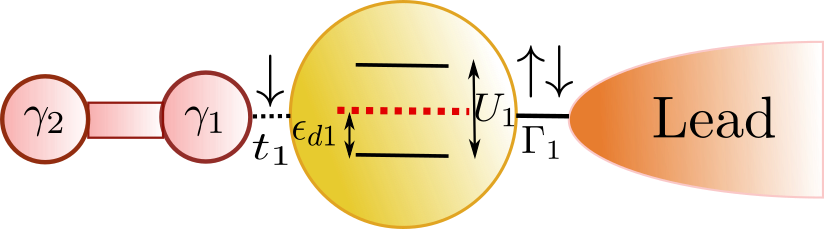
\includegraphics[scale=0.6]{IMAGES/Majorana/QD-M.png}
    \caption{\label{fig:ModelM-QD} Model for the QD-Majorana system. Solid lines: Hopping interactions: $V_1$ couplings of QD1 . Dashed lines: Majorana spin-$\dw$ effective couplings \eqref{eq:MajoranaCoupling} $t_1$. The atomic energy levels appear inside each QD $\ep_1$ are tuned by the gate voltages. The coulomb interaction is represented by $U_1$ separates two energy levels.  The red dashed horizontal lines represent the Fermi level. }
\end{figure}

The Hamiltonian for Majorana-QD-lead hybrid system (See \ref{fig:ModelM-QD}) is  given by
\begin{equation}
    H=H_{QD-Lead}+H_{M-QD}+H_M.
\end{equation}
Where $H_{QD-Lead}$ is the Hamiltonian for the non-interacting Anderson model \eqref{eq:Anderson}, $H_M$ is the Hamiltonian of the Majorana chain and $H_{M-QD}$ represents the coupling between the QD and the Majorana Fermion at the boundary.

Now, the real question is how to define the coupling between the QD and the MBS. In fact, there are many ways to represent this interaction. One alternative is to replace in $H_{M}$ with the entire Kitaev chain Hamiltonian \eqref{eq:kitaevHam} (or  even with the  Majorana chain \eqref{eq:MajoranaChainHam}) and then pick $H_{M-QD}$ as the coupling between the QD and the first site of the chain \cite{vernek_subtle_2014}.  A simpler approach is  to define an effective coupling with the Majorana operator at the edge of the Majorana chain. Since the Kitaev chain is spin-less, we choose to couple the Majorana to the spin-$\dw$ channel of the QD \footnote{An appropriate justification of this fact can be found in \cite{ruiz-tijerina_interaction_2015}} . Therefore, the Majorana fermion should be the superposition of the creation and annihilation operators of a spin $\dw$ particle $f_\dw$:

\begin{equation}
\gamma_1 := \frac{1}{\sqrt{2}} \left( f^\dagger_{\dw} + f_{\dw}\ \right) , \gamma_2 := \frac{1}{\sqrt{2}} \left( f^\dagger_{\dw} - f_{\dw} \right).
\end{equation}


This makes possible to define an effective coupling between the Majorana Mode and the dot by attaching $\gamma_1$ with the spin-$\dw$ channel in the QD

%H_{TS} & = & 2\epsilon_{m}\gamma_{1}\gamma_{2}\nonumber \\
\begin{eqnarray}
H_{M-QD} & = &  t_1 \left(d_{\downarrow}^{\dagger}\gamma_{1}+\gamma_{1}d_{\downarrow}\right) .
% \\
% & = &  \sum_{i}t_{i} \left(d_{i\downarrow}^{\dagger}f^\dagger_{\dw} + 
% f_{\downarrow}d_{i\dw} +d_{i\downarrow}^{\dagger}f_{\dw}+
% +f_{\downarrow}^{\dagger} d_{i\downarrow}\right).
\label{eq:MajoranaCoupling}
\end{eqnarray}
\noindent In addition, the two Majoranas at the edges of the chain can have an internal coupling 
\begin{equation}
H_M = \epsilon_M  \gamma_1\gamma_2. 
\end{equation}
\noindent According to Kitaev's initial paper \cite{kitaev_unpaired_2001}, this coupling term decreases exponentially with the length of the chain. This explains why this term is not taken into account in many computations. 


% \begin{equation}
%     \omega\Green{A,B} =\delta_{A^{\dagger},B}+\Green{\left[A,H\right],B}
% \end{equation}

Replacing the Dirac fermion operators we obtain the following Hamiltonians 

\begin{eqnarray}
H_{M} & = & \epsilon_{m}f_{\downarrow}^{\dagger}f_{\downarrow},\\
H_{M-QD}&=&\frac{t_1}{\sqrt{2}}d_{1\downarrow}^{\dagger}f_{\downarrow}+\frac{t_1^{*}}{\sqrt{2}}f_{\downarrow}^{\dagger}d_{1\downarrow}+\frac{t_1}{\sqrt{2}}d_{1\downarrow}^{\dagger}f_{\downarrow}^{\dagger}+\frac{t_1^{*}}{\sqrt{2}}f_{\downarrow}d_{1\downarrow}.
\end{eqnarray}

\noindent Finally we have the Hamiltonian

\begin{equation}
H =\sum_{k,\sigma}\left(\epsilon_1+\frac{U_1}{2}\right)d_{1\sigma}^{\dagger}d_{1\sigma}+ \frac{U}{2}(d_{1\sigma}^{\dagger}d_{1\sigma}-1)^{2} + t_1 d_{1\downarrow}^{\dagger}\gamma_{1} + Vd^\dagger_{1\sigma}c_{k\sigma}+ \epsilon_{m}f_{\downarrow}^{\dagger}f_{\downarrow} + \text{h.c}.
\label{eq:QD-Mham}
\end{equation}


\noindent The fidelity of this effective model has been discussed by \citet{ruiz-tijerina_interaction_2015}
concluding that this model reproduces the
same results than coupling a  Kitaev chain model in the topological phase to a QD.
(This statement is true even for more realistic models of the TS including Rashba spin-orbit interactions and a Zeeman field \citep{ruiz-tijerina_interaction_2015}
).\\


\section{Non-interacting QD coupled to  Majorana chain \label{sec:GreenMaj-DQD}}

In the non-interacting case we can use the ballistic transport equations from \ref{sec:transport}.The green functions are then determined by the following set of linear equations. 




\begin{align}
    \left(\omega-\epsilon_{M}\right)\Green{f_{\downarrow},d_{1\downarrow}^{\dagger}}&=\left(\omega+\epsilon_{M}\right)\Green{f_{\downarrow}^{\dagger},d_{1\downarrow}^{\dagger}}=\frac{t^*_1}{\sqrt{2}}\left(\Green{d_{1\downarrow},d_{1\downarrow}^{\dagger}}-\Green{d_{1\downarrow}^{\dagger},d_{1\downarrow}^{\dagger}}\right) \label{eq:QDM1} \\ 
    \left(\omega-\epsilon_{1}\right)\Green{d_{1\downarrow},d_{1\downarrow}^{\dagger}}&=1+\frac{t_1}{\sqrt{2}}t_{1}\Green{f_{\downarrow},d_{1\downarrow}^{\dagger}}+\frac{t_1}{\sqrt{2}}t_{1}\Green{f_{\downarrow}^{\dagger},d_{1\downarrow}^{\dagger}}+V_{1}\sum_{\mathbf{k}}\Green{c_{\mathbf{k\downarrow}},d_{1\downarrow}^{\dagger}} \label{eq:QDM2} \\ 
    \left(\omega-\epsilon_{\mathbf{k}}\right)\Green{c_{\mathbf{k}},d_{1\downarrow}^{\dagger}}&=V_{1}^{*}\Green{d_{1\downarrow},d_{1\downarrow}^{\dagger}}\label{eq:QDM3} \\
    \left(\omega+\epsilon_{1}\right)\Green{d_{1\downarrow}^{\dagger},d_{1\downarrow}^{\dagger}}&=-\frac{t_1}{\sqrt{2}}\Green{f_{\downarrow},d_{1\downarrow}^{\dagger}}-\frac{t_1}{\sqrt{2}}\Green{f_{\downarrow}^{\dagger},d_{1\downarrow}^{\dagger}}-V_{1}^{*}\sum_{\mathbf{k}}\Green{c_{\mathbf{k\downarrow}}^{\dagger},d_{1\downarrow}^{\dagger}} \label{eq:QDM4} \\
    \left(\omega+\epsilon_{\mathbf{k}}\right)\Green{c^\dagger_{\mathbf{k}},d_{1\downarrow}^{\dagger}}&=-V_{1}^{*}\Green{d_{1\downarrow},d_{1\downarrow}^{\dagger}}. \label{eq:QDM5}
\end{align}

The graph representing these green functions is in \ref{fig:green-M-QD} (a)  (Look \ref{sec:GraphMethod} for details). However, using that $\left(\omega-\epsilon_{M}\right)\Green{f_{\downarrow},d_{1\downarrow}^{\dagger}}=\left(\omega+\epsilon_{M}\right)\Green{f_{\downarrow}^{\dagger},d_{1\downarrow}^{\dagger}}$ we can take
 $\Green{f_{\downarrow}^{\dagger},d_{1\downarrow}^{\dagger}}$ out of the equations. After eliminating this term from \eqref{eq:QDM2} it becomes
 
 \begin{align}
\left(\omega-\epsilon_{1}\right)\Green{d_{1\downarrow},d_{1\downarrow}^{\dagger}}&=1+\frac{t_{1}}{\sqrt{2}}\left(1+\frac{\omega-\epsilon_{M}}{\omega+\epsilon_{M}}\right)\Green{f_{\downarrow},d_{1\downarrow}^{\dagger}}+V_{1}\sum_{\mathbf{k}}\Green{c_{\mathbf{k\downarrow}},d_{1\downarrow}^{\dagger}} \\
&=1+\frac{\sqrt{2}t_{1}}{\omega+\epsilon_{M}}\Green{f_{\downarrow},d_{1\downarrow}^{\dagger}}+V_{1}\sum_{\mathbf{k}}\Green{c_{\mathbf{k\downarrow}},d_{1\downarrow}^{\dagger}}.
\end{align}

\noindent Similarly, 

\begin{equation}
    \left(\omega+\epsilon_{1}\right)\Green{d_{1\downarrow}^{\dagger},d_{1\downarrow}^{\dagger}}=-\frac{\sqrt{2}t_{1}}{\omega+\epsilon_{M}}\Green{f_{\downarrow},d_{1\downarrow}^{\dagger}}-V_{1}^{*}\sum_{\mathbf{k}}\Green{c_{\mathbf{k\downarrow}}^{\dagger},d_{1\downarrow}^{\dagger}}.
\end{equation} 
 
 
 With these new equations we can construct the graph is  in \ref{fig:green-M-QD} (b) .  Using the Graph-Gauss-Jordan algorithm from \ref{sec:Algorithm}  we proceed to eliminate vertexes $c_k$ , $c_k^\dagger$ and $d_1^\dagger$ in that order. The result is the graph in figure \ref{fig:green-M-QD}(c) with 
 
 \begin{figure}[t]
    \centering
    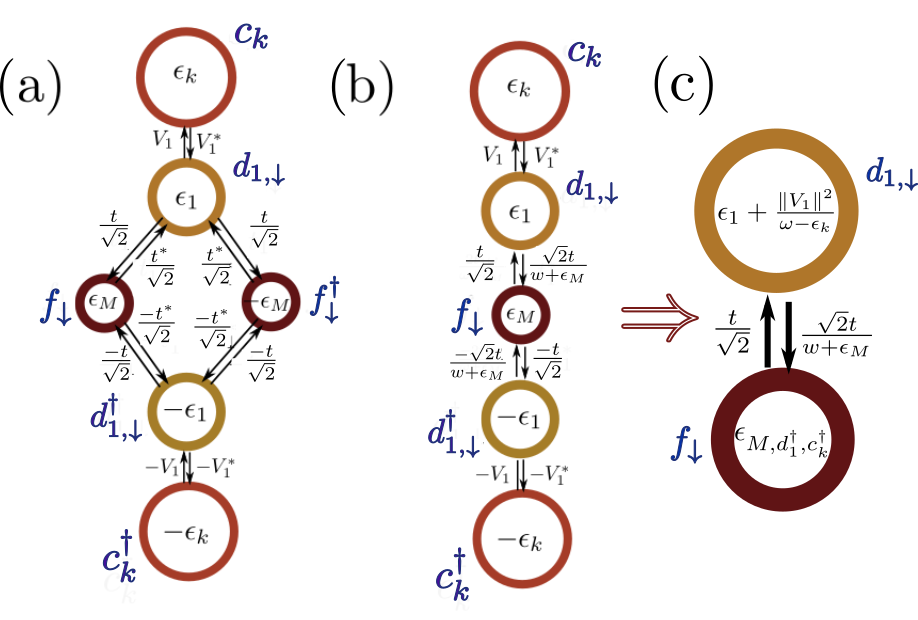
\includegraphics[scale=0.5]{IMAGES/Graphs/Grenn-Majorana.png}
    \caption{ \label{fig:green-M-QD} Graph $\GM$ representing the transport equations.   \protect\Source{}}
\end{figure}
 
 \begin{equation}
    \epsilon_{M,d_1^\dagger,c^\dagger}= \epsilon_{M}+\frac{\omega}{\omega+\epsilon_{M}}\frac{\left\Vert t\right\Vert ^{2}}{\omega+\epsilon_{1}+\sum_{\mathbf{k}}\frac{V_{1}V_{1}^{*}}{\omega+\epsilon_{\mathbf{k}}}}.
\end{equation}
 
 \noindent We finally eliminate $f_\dw$ to obtain 
 
\begin{equation}
    \Green{d_{1\downarrow},d_{1\downarrow}^{\dagger}}=\left[\omega-\epsilon_{1}-\sum_{\mathbf{k}}\frac{V_{1}V_{1}^{*}}{\omega-\epsilon_{1}}-\frac{\omega}{\omega+\epsilon_{M}}\frac{\left\Vert t\right\Vert ^{2}}{\omega -\epsilon_{M,d_1^\dagger,c^\dagger}}\right]^{-1}.
\end{equation}
% Hence we just need the green function of $\GreenG{f_{\downarrow},f_{\downarrow}^{\dagger}}{\GM-d_{1}}$ removing $d_1$ out of the graph. This case is much simpler since $f_\downarrow$ is just attached to $d^\dagger_1$ . Thus we get
% \begin{equation}
%     \GreenG{f_{\downarrow},f_{\downarrow}^{\dagger}}{\GM-d_{1}}=\left[\omega-\epsilon_{M}-\frac{\omega}{\omega+\epsilon_{M}}\frac{\left\Vert t\right\Vert ^{2}}{\omega+\epsilon_{1}-\sum_{\mathbf{k}}\frac{V_{1}V_{1}^{*}}{\omega-\epsilon_{\mathbf{k}}}}\right]^{-1}.
% \end{equation}

\noindent This is the Green function we have been looking for. After a few algebraic operations it is possible to show that this result is equivalent to the first computation done by \citeauthor{liu_detecting_2011}  in the paper \cite{liu_detecting_2011}. 




To compute the DOS we need to replace $\sum \frac{V_1V^*_1}{\omega -\epsilon_k}= -i\Gamma_1$ as we already did in \ref{sec:GraphMethod}. Note that these computations are only for the spin-$\dw$ channel. The spin-$\up$ channel is even simpler since this channel is not coupled to the Majorana mode by convention. Hence it corresponds to the case of a single quantum dot coupled to a Lead.  The results for the DOS can be observed in \ref{fig:M1-Tot}. Each figure has an inset showing the model in the Majorana representation. The small blue and red balls are Majorana fermions just as the ones in figure \ref{fig:top.phases kitaev}. The Majorana at the edge of the  chain is represented by the isolated red ball connected to the QD (Figure \ref{fig:M1}). The isolated blue ball in Figure\ref{fig:M1-em} represents the Majorana at the other edge of the chain which is connected to the sphere by the parameter $\epsilon$. 



\begin{itemize}
    \item\textbf{ \ref{fig:M1-Tot}.(a),(b):}  The spin-$\up$ DOS shows the result of coupling the QD with the lead and without Majoranas. When the parameter $t$ is increased, the MZM is coupled to the spin-$\dw$ which causes the dispersion of the DOS. The most relevant signature is the robust height of $0.5$  in the DOS that is observed in the central peak for all $t>0$. This mid-height DOS is responsible for the decay of half a quanta in the conductivity of the QD \cite{liu_detecting_2011}.
    % In addition we observe that two new states emerge at $\omega \sim t^2$ caused 

    \begin{figure}[h]
     \centering
    \subfloat[Tuning the Majorana coupling $t_1$ \label{fig:M1}]{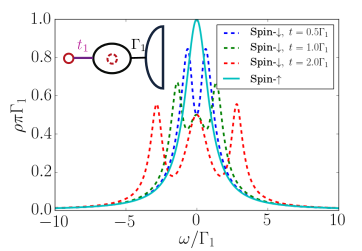
\includegraphics[scale=0.73]{IMAGES/Majorana/M1.png}}
     \subfloat[Tuning dot's gate voltage $\ep_1$ \label{fig:M1-e1}]{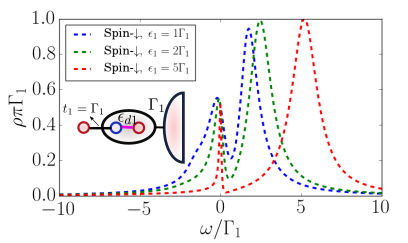
\includegraphics[scale=0.73]{IMAGES/Majorana/M1-e1.png}}  \\
    \subfloat[Tuning $\ep_M$ \label{fig:M1-em}]{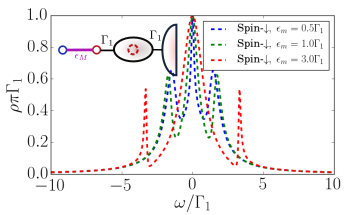
\includegraphics[scale=0.75]{IMAGES/Majorana/M1-eM.png}}
    
     \caption{Density of states for a Majorana coupled to a QD under the tuning of different parameter. The tuning parameter is drawn in purple line in the inset model.  \label{fig:M1-Tot} \protect\Source{   }}
\end{figure}

  
    \item\textbf{ \ref{fig:M1-Tot}.(c),(d):} This time a gate voltage is induced in the dot which breaks PHS. However the robust $0.5$-height Majorana signature prevails in the dot even at very high gate voltages where the dot is expected to be empty. This result is similar to the one in \cite{vernek_subtle_2014}, where the is attached to the last cite of the Kitaev chain. 
    
    \item\textbf{ \ref{fig:M1-Tot}.(e),(f):} The term $\epsilon_M$ couples both Majoranas at the edges of the chain. The strength of this parameter decays exponentially with the length of the Majorana  chain so that it is often neglected . Here we observe the consequences of including this parameter in the model. The spin-$\dw$ DOS for energies $\omega < \ep_M$ is forced to take the same value of the the spin-$\up$ DOS. This clearly destroys the Majorana zero mode in the dot.   
\end{itemize}







\section{Kondo-Majorana physics}
\begin{figure}[t]
\centering
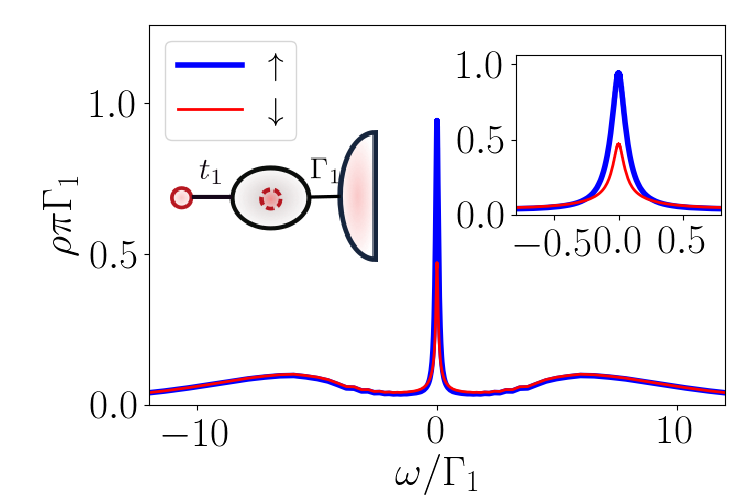
\includegraphics[scale=0.6]{IMAGES/Majorana/NRG_M1.png}
\caption{ \label{fig:NRG-1M} DOS at $t_1 = \Gamma_1$ at the PHS-point.  Insets: Left: QD-Majorana model. Right: Zoom to low energy DOS. \protect\Source{.}}
\end{figure}

In interacting quantum dots the Kondo effect is visible at low temperatures even when the QD is attached to a Majorana chain, which allows the study Kondo-Majorana physics. To observe this , we used the NRG code with a fixed Coulomb repulsion of $U = 17.6\Gamma_1$, just as in section \ref{sec: NRG-DQD}. Then, particle-hole equilibrium is achieved when $\left(\epsilon_{1}+\frac{U_1}{2}\right)\hat{n}_{1\sigma}$. Any tunning of the dot's gate voltage must be understood as a displacement $\Delta \epsilon_1$ from this equilibrium point. 




 \begin{figure}[h]
 \centering
   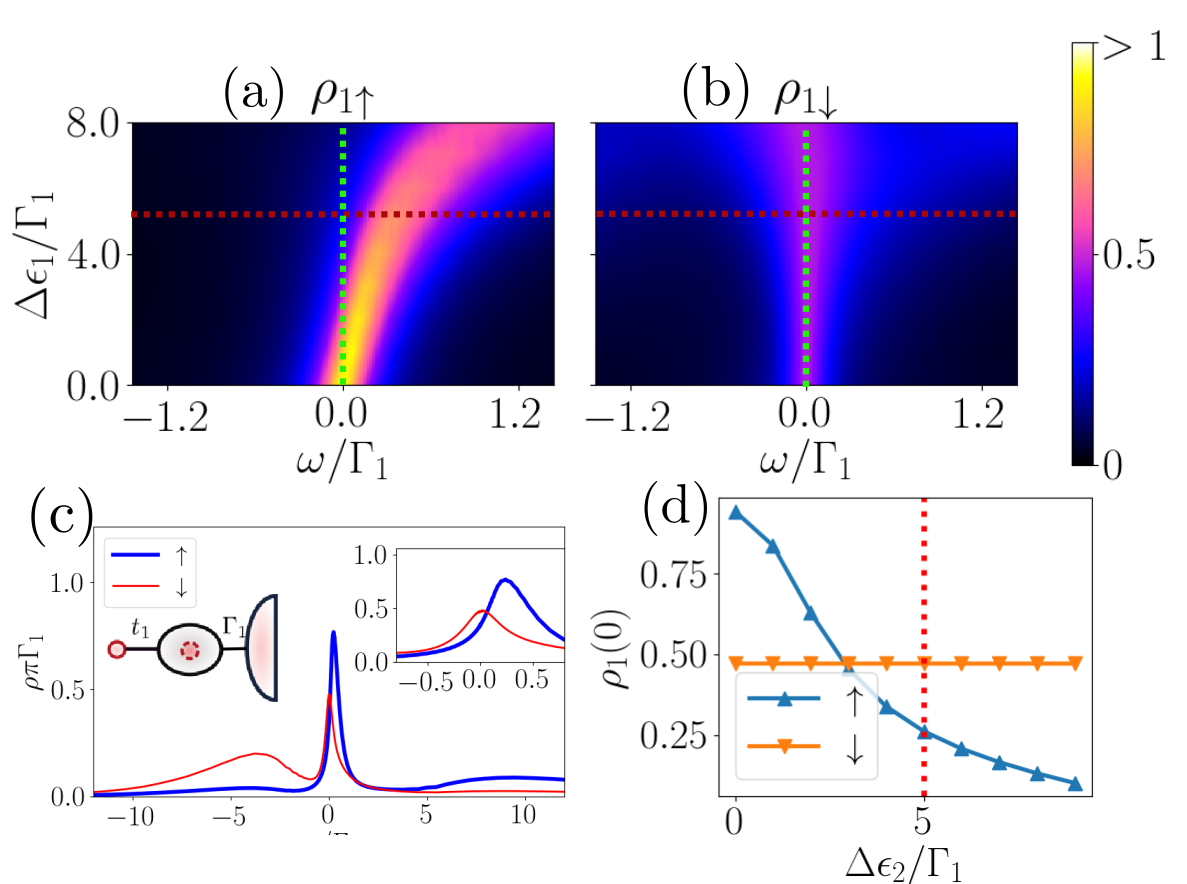
\includegraphics[scale=0.57]{IMAGES/Majorana/NRG-FullED.png}
   \caption{ \label{fig:QD-ed}(a)\&(b): Dependence of the DOS over the gate voltage $\Delta \epsilon_1$ at $t_1 = \Gamma_1$. (a)Spin-$\up$ (b) Spin-$\dw$. (c) DOS at the red-dashed horizontal cut in (a)\&(b). Insets: Left: QD-Majorana model. Right: Low energy DOS. (d) DOS at the Green-dashed vertical cut in (a)\&(b). \protect\Source{.} }
 \end{figure}



 \ref{fig:NRG-1M} shows the PHS case for a Majorana coupling $t_1=\Gamma_1$. The two small wide peaks at the borders of the plot are the coulomb states. In the right inset of the figure, we observe the low-temperature regime inside the gap. There, two zero modes can be appreciated.  While the spin-$\up$ DOS is the same Kondo peak from Figure \ref{fig:NRG-1D}, the spin-$\dw$ DOS reveals a Majorana zero mode of half the amplitude of the Kondo peak $\left(\frac{0.5}{\pi\Gamma_1}\right)$.  This  Majorana signature resembles the one in Figure \ref{fig:M1}.
 \begin{figure}[H]
 \centering
 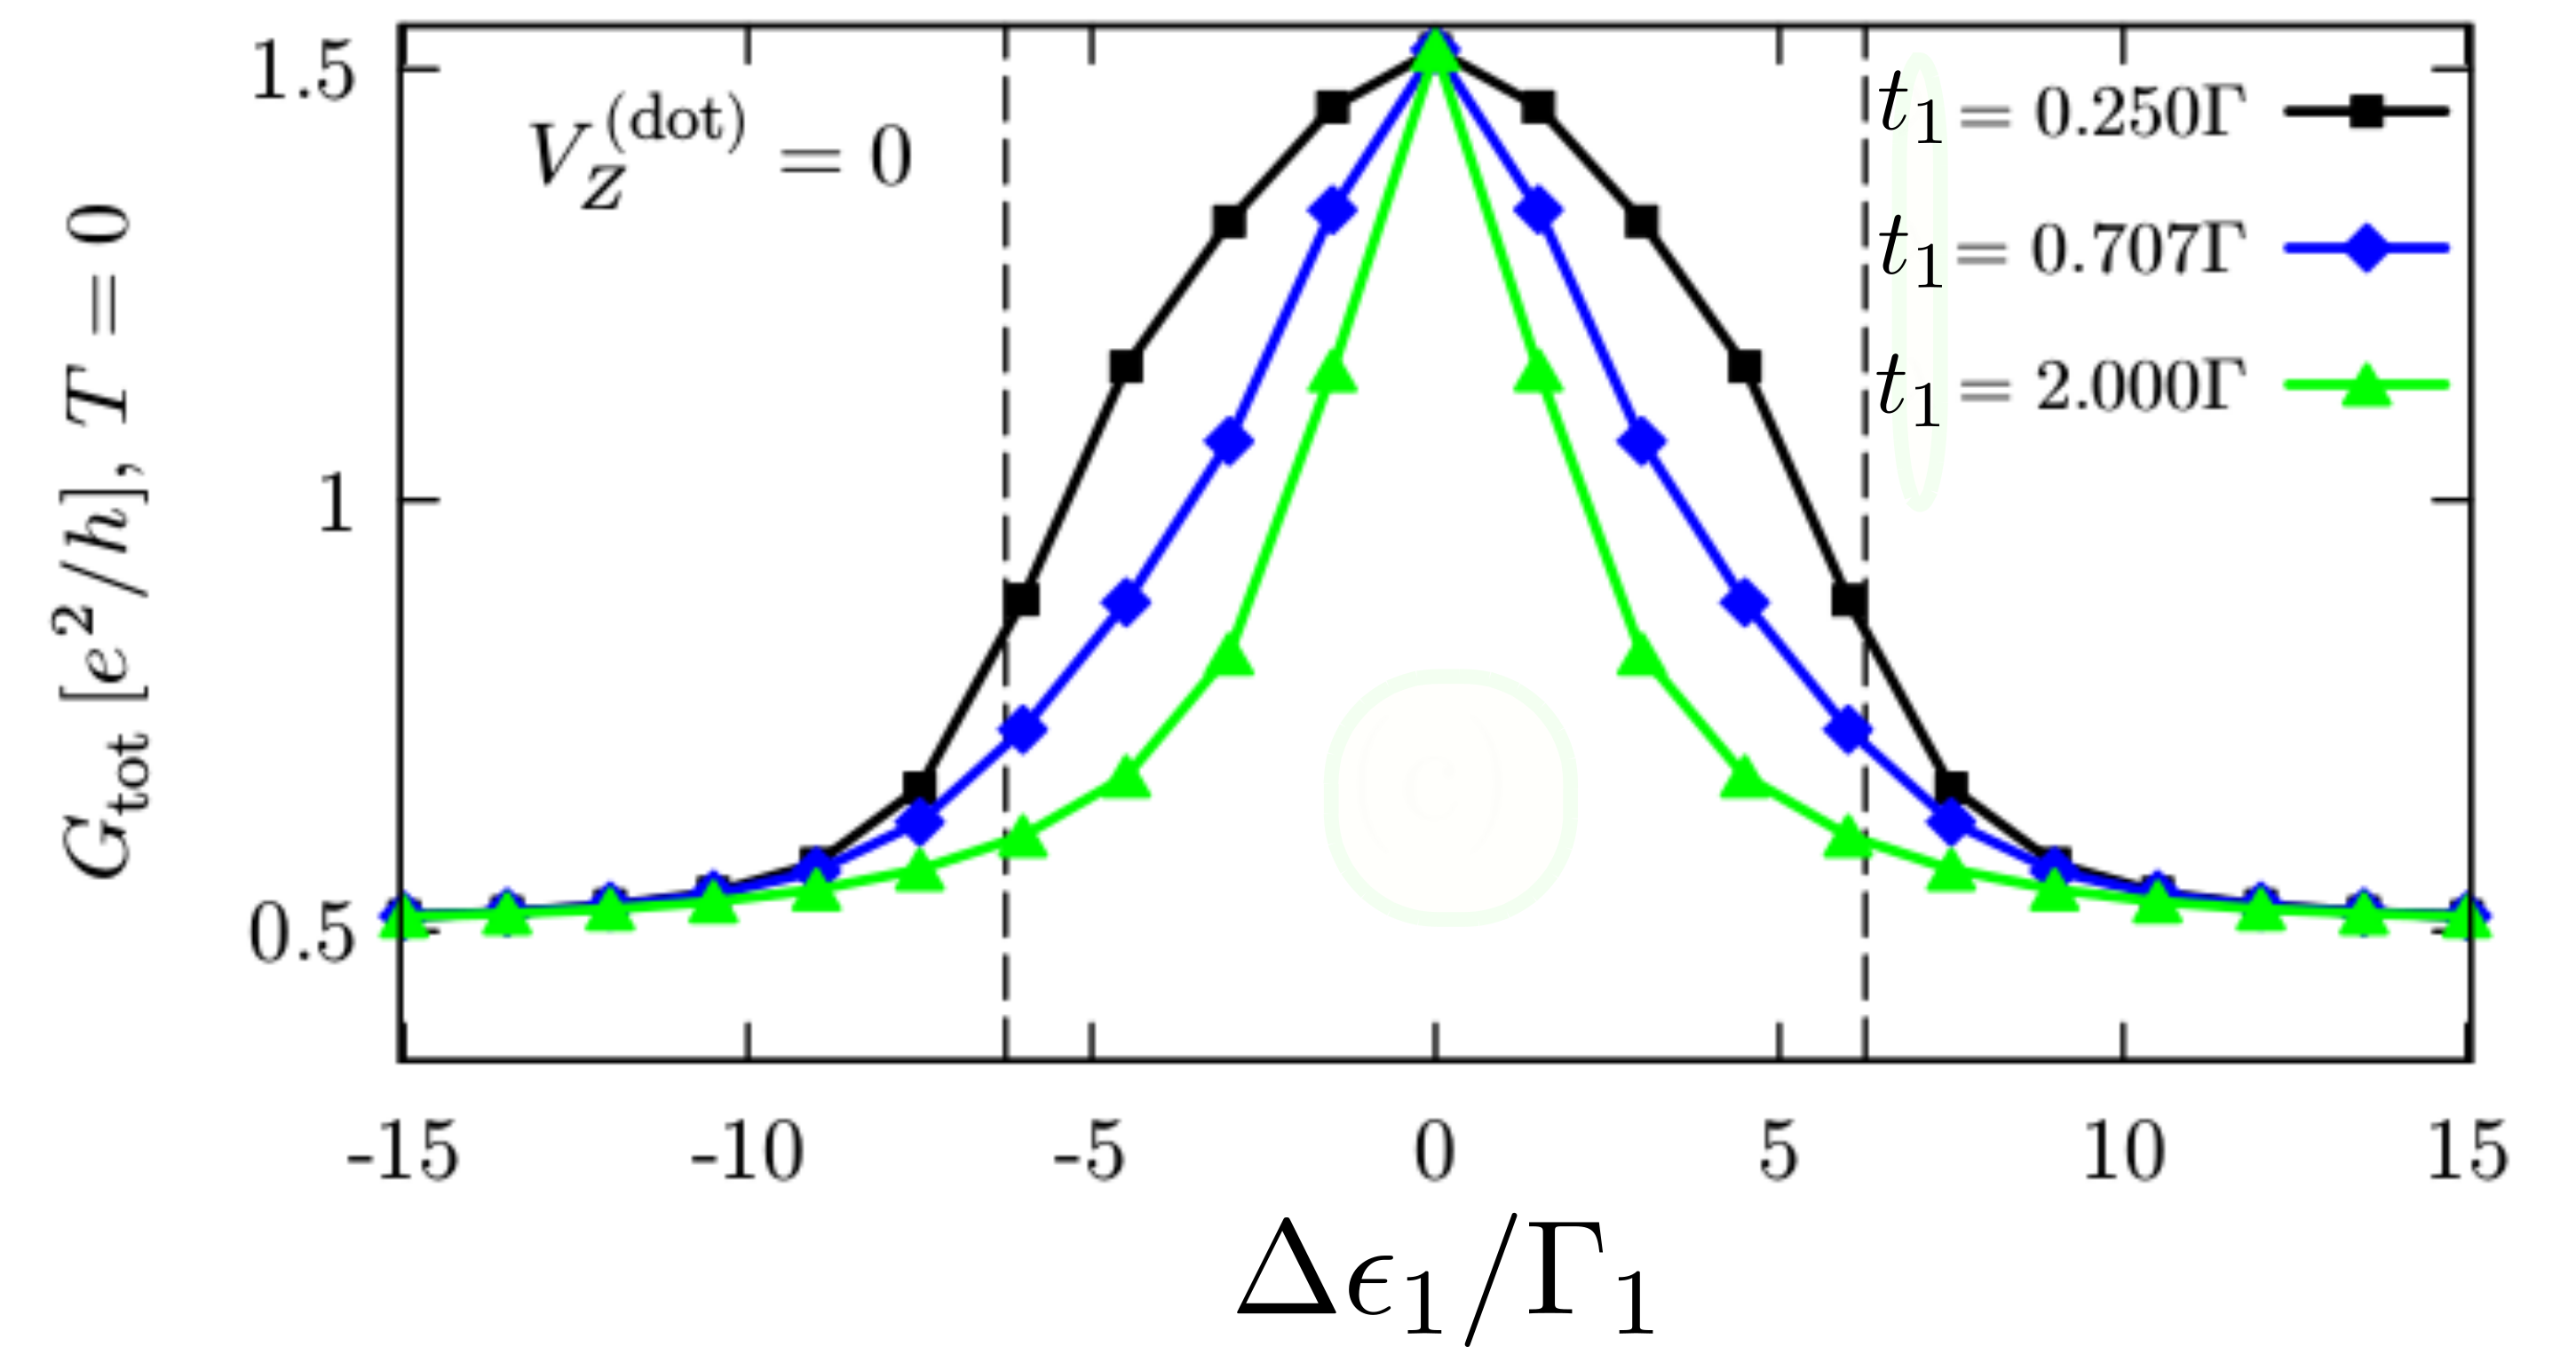
\includegraphics[scale=0.48]{IMAGES/Majorana/Luis.png}
 \caption{\label{fig:Luis}Dependence of the zero-bias conductance over tuning voltage \protect\Source{Adapted from \cite{ruiz-tijerina_interaction_2015}.}}
 \end{figure}


 It is possible to separate Kondo and Majorana physics by inducing a gate voltage in the dot. As observed in \ref{fig:QD-ed}(a), the gate voltage detunes the Kondo peak from the Fermi energy. Instead, the MZM in \ref{fig:QD-ed}(b) remains at the same position. At $\Delta \epsilon_1 = 5\Gamma_1$ we can already observe a decaying Kondo peak next to the robust Majorana signature of height $\frac{0.5}{\pi\Gamma}$ (\ref{fig:QD-ed}(c)). This is more clear in \ref{fig:QD-ed}(d) where the spin-$\up$ DOS decays with $\Delta \ep_1$ while the spin-$\dw$ DOS is stable, even at $\Delta \ep_1 \sim \frac{U}{2} = 8.6$ where the dot is supposed to be empty. 


% the observecharacterized by the the Majorana in the spin-$\dw$ channel will produce a peak at the fermi energy of half of the amplitude of the Kondo peak  This will be our Majorana signature. 


 This interesting result was already pointed out by  \citeauthor{ruiz-tijerina_interaction_2015}  
 who proved that increasing the gate voltage would produce a visible decay in the the zero bias conductance down to $\frac{0.5 e^2}{h}$ (See \ref{fig:Luis}). Hence, allowing to measure the Majorana signature without the superposition with the Kondo peak.  This result is clear from \ref{fig:QD-ed}. At $\Delta \epsilon = 0$ the DOS at the Fermi energy is $\frac{1}{\pi \Gamma_1}$ for spin-$\up$ and $\frac{0.5}{\pi \Gamma_1}$ for spin-$\down$. Instead, for bigger values of $\Delta \epsilon_1$  only the $\frac{0.5}{\pi \Gamma_1}$-height spin-$\dw$ peak appears.  Since the zero bias conductance at zero temperature is essentially the sum of both spectral densities (times unit correction), \ref{fig:QD-ed} recovers the results in \ref{fig:Luis}. 

 

 % \citeauthor{ruiz-tijerina_interaction_2015} also demonstrates that it is possible to  is 

Another possibility to distinguish Kondo and Majorana physics is quenching the Kondo effect with a strong magnetic field . Similar to what was observed in \ref{fig:Luis}, the Kondo peak will be destroyed while the Majorana signature remains stable \cite{ruiz-tijerina_interaction_2015}. 

In the next chapter we will use the ideas from this chapter to study the model of a DQD attached to a Majorana zero mode.



% \subsection{State-of-the-art and prospective applications}

% The possibility of using QD's in the pursuit of Majorana quasi-particles has attracted considerable attention in the last few years. The observation of Kondo signatures in QD-superconductor heterostructures \cite{deng_anomalous_2012} has motivated the study of Kondo-Majorana co-existance in QDs \cite{ruiz-tijerina_interaction_2015,gorski_interplay_2018} and non-fermi liquid behavior \cite{zitko_quantum_2011}. In addition, the precise experimental experimental control over QDs has opened the possibility of implementing scalable braiding proposals \ref{fig:braid}(a) and  quantum architectures for topological quantum computation \ref{fig:braid}(b). 

% These architectures perform adiabatic evolutions similar to the ones described in  \ref{subsec:non-ab} to braid Majorana fermions. This operation strongly relies on the possibility of manipulating the Majorana zero modes inside the dots. The mean idea of MZM manipulation is to  tune the gate voltage of one dot to induce the Majoranas to "move" into the other dots.  In a prospective braiding protocol, as the one described in  \cite{malciu_braiding_2018} (\ref{fig:braid}(a)), this manipulation process would have to be performed several times. However, till this moment MZM manipulation hasn't been achieved experimentally. 


% Notwithstanding, the future for this area is still very promising. Recent experiments have documented the observation of Majorana signatures in Majorana-QD devices \cite{deng_majorana_2016} and Andreev molecules in topological superconductors attached to double quantum dots \cite{su_andreev_2017}. The next steps are clearly directed to achieve Majorana manipulation. The simplest device where this process is possible is in a double quantum dot (DQD). This fundamental case is the mean objective of this thesis and will be treated in the following chapter. 

% \begin{figure}[H]
%   \centering
%   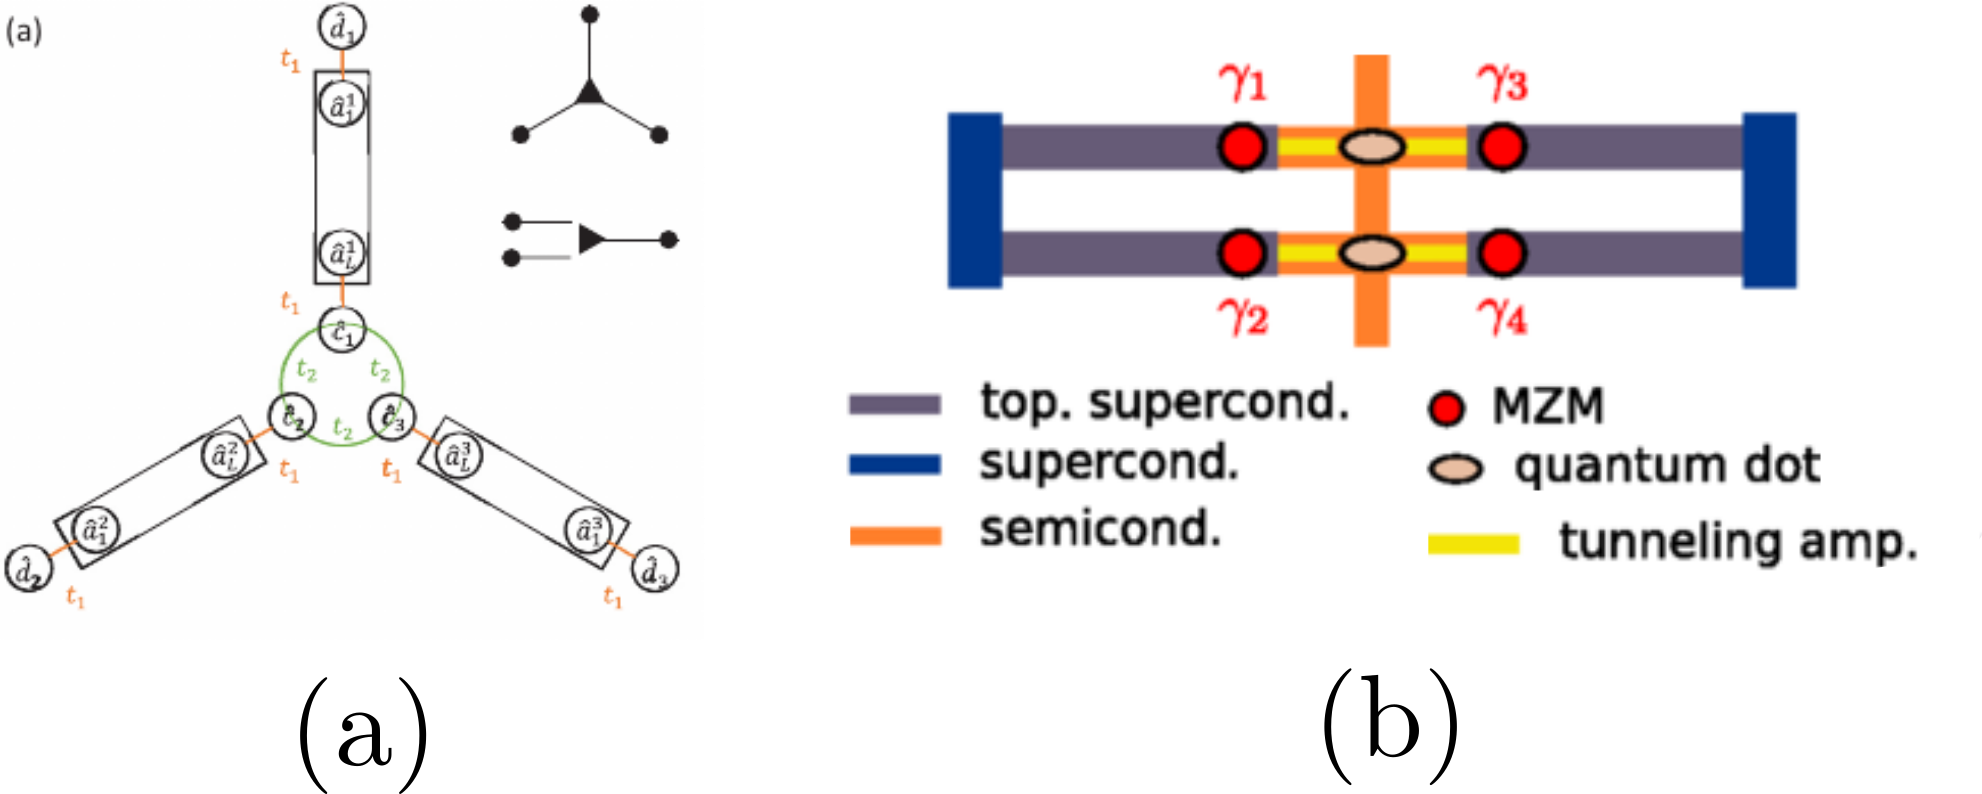
\includegraphics[scale=1]{IMAGES/Majorana/Prospective.png}
%   \caption{\label{fig:braid} a) Braiding proposal b) Basic architecture with four Majorana Zero Modes in a scalable quantum computer.\protect\Source{Adapted from (a) \cite{malciu_braiding_2018} (b) \cite{karzig_scalable_2017} .}}
% \end{figure}




% \begin{eqnarray*}
% H_{TS} & = & 2\epsilon_{m}f_{\downarrow}^{\dagger}f_{\downarrow}-\epsilon_{m}\\
% H_{int} & = & \sum_{i}\tilde{t_{i-}}d_{i\downarrow}^{\dagger}f_{\downarrow}+\tilde{t_{i-}}^{*}f_{\downarrow}^{\dagger}d_{i\downarrow}+\tilde{t_{i+}}d_{i\downarrow}^{\dagger}f_{\downarrow}^{\dagger}+\tilde{t_{i+}}^{*}f_{\downarrow}d_{i\downarrow}
% \end{eqnarray*}

% with $\tilde{t}_{i\pm}=\frac{1}{\sqrt{2}}\left(\left|t_{i1}\right|-i\left|t_{i1}\right|e^{i\phi_{i}}\right).$



% so that 

% \[
% \gamma_{1}=\frac{1}{\sqrt{2}}\left(f_{\downarrow}^{\dagger}+f_{\downarrow}\right)\ ,\gamma_{2}=\frac{1}{i\sqrt{2}}\left(f_{\downarrow}^{\dagger}-f_{\downarrow}\right).
% \]


% \begin{eqnarray}
% H_{TS} & = & 2\epsilon_{m}\gamma_{1}\gamma_{2}\nonumber \\
% H_{int} & = & \sum_{i}t_{i1}\left(d_{i\downarrow}^{\dagger}\gamma_{1}+\gamma_{1}d_{i\downarrow}\right)+it_{i2}\left(d_{i\downarrow}^{\dagger}\gamma_{2}+\gamma_{2}d_{i\downarrow}\right),\label{eq:Majorana-ham}
% \end{eqnarray}


% where $\gamma_{1,2}$are the two Majorana operators and$t_{i1,2}$
% are the hopping terms between the Majoranas and the QDs.




% A Majorana chain coupled to a QD can be studied using the methods described in chapter \ref{chap: Methods}






% % where $H_{d_{i}}$is the QD hamiltonian for dot $i$ \prettyref{eq:DotHam}
% % ,$t$ is the hopping term between both dots, $H_{int}$is the dot-TS
% % interaction and $H_{TS}$ is the TS-hamiltonian . In \citep{vernek_subtle_2014},
% % the TS is modeled as a Kitaev chain \citep{kitaev_unpaired_2001}
% % and $H_{int}$ is the hopping interaction between dots and chain 

% \begin{eqnarray}
% H_{TS} & = & -\sum_{j=1}^{N}\mu a_{j}^{\dagger}a_{j}+\sum_{j=1}^{N-1}\left[-t'(a_{j}^{\dagger}a_{i+1}+a_{j+1}^{\dagger}a_{j})+\Delta a_{j}a_{j+1}+\Delta^{*}a_{j+1}^{\dagger}a_{j}^{\dagger}\right]\nonumber \\
% H_{int} & = & \sum t_{i}d_{i\downarrow}^{\dagger}a_{1}+t_{i}^{*}a_{1}^{\dagger}d_{i\downarrow},\label{eq:Kitaev-dot}
% \end{eqnarray}


% where $a_{j}^{\dagger}$is the creation operator at site $j$ of the
% chain, $t'$ is the hopping term between consecutive sites, $\Delta$
% is the superconducting gap and $t_{i}$ is the hopping interaction
% between the dot $i$ and the first site of the chain. We also assume
% the dot only interact with spin-down $\downarrow$ operators in the
% chain. \\

% Using a Green's function approach on \prettyref{eq:Kitaev-dot} ,
% \citet{vernek_subtle_2014} concludes that the Majorana mode at the
% end of the chain leaks inside the QD when the TS is in the topological
% phase . This fact favors a more simple effective model that has been
% used in literature for simulation QD-TS interactions \citep{liu_detecting_2011,golub_kondo_2011,lee_kondo_2013}.
% The model consists in considering only the coupling between the dots
% and the Majorana modes that emerge in the topological phase. The resulting
% hamiltonian is 



% \[
% f_{\downarrow}^{\dagger}=\frac{1}{\sqrt{2}}\left(\gamma_{1}-i\gamma_{2}\right)\ ,\ f_{\downarrow}=\frac{1}{\sqrt{2}}\left(\gamma_{1}+i\gamma_{2}\right)
% \]


% so that 

% \[
% \gamma_{1}=\frac{1}{\sqrt{2}}\left(f_{\downarrow}^{\dagger}+f_{\downarrow}\right)\ ,\gamma_{2}=\frac{1}{i\sqrt{2}}\left(f_{\downarrow}^{\dagger}-f_{\downarrow}\right).
% \]


% Supposing $t_{i1}=\left|t_{i1}\right|$ and $t_{i2}=\left|t_{i2}\right|e^{i\phi_{i}}$
% to have a $\phi_{i}$-phase with respect to $t_{i1}$, we get to the
% following hamiltonian 



% \begin{eqnarray}
% H_{TS-2QDs} & = & H_{d_{i}}+\sum_{\sigma}\left(td_{1\sigma}^{\dagger}d_{2\sigma}+t^{*}d_{1\sigma}^{\dagger}d_{2\sigma}\right)\nonumber \\
%  &  & \ \enskip\ \enskip+\sum_{i}\left[\tilde{t_{i-}}d_{i\downarrow}^{\dagger}f_{\downarrow}+\tilde{t_{i-}}^{*}f_{\downarrow}^{\dagger}d_{i\downarrow}+\tilde{t_{i+}}d_{i\downarrow}^{\dagger}f_{\downarrow}^{\dagger}+\tilde{t_{i+}}^{*}f_{\downarrow}d_{i\downarrow}\right]+2\epsilon_{m}f_{\downarrow}^{\dagger}f_{\downarrow}-\epsilon_{m}.\label{eqFinalMJ-2QDs}
% \end{eqnarray}


% \bibliography{Majorana-QD,Kitaev-Majorana,Kondo}